% Chapter Template

\chapter{Introduction} % Main chapter title

\label{Chapter1} % Change X to a consecutive number; for referencing this chapter elsewhere, use \ref{ChapterX}

%----------------------------------------------------------------------------------------
%	SECTION 1
%----------------------------------------------------------------------------------------

\section{Introduction}

The Influence of IoT-Devices in everyday life has been rising for decades.
Connected devices are expected to number 20 billion \parencite{gartner0} by 2020 in nearly every industry.
According to \parencite{verizon} the use of media and entertainment on digital devices increased by 120 \% in 2016 compared to 2013,
the industry was third in terms of accepting IoT,
with manufacturing (204\%) and finance and insurance (138\%) industries topping the chart.

Within the entertainment industry, escape rooms have been a growing sector since the first escape room launched 2007 in Japan.
Escape rooms generally follow the same structure: People are locked into a room, have to solve riddles,
and get out in a defined period or will be freed by a supervisor who watches the process to support
and step in in case of an emergency.

This field offers lots of possibilities for technical development, be it the use of different sensors, the use of Virtual Reality or flexible story-telling (depending on the users actions).
In this thesis, my goal was to make the first step to a smart escape room.

The faculty provided an escape room with micro-controllers as riddles.
The room provided support for the existing riddles but provided little support for changes.
This thesis will focus on developing an easy integration system for new riddles from different devices.
Furthermore, a User Interface which supports communication with existing and new riddles dynamically was developed.
The first chapter will provide an overview about our research on topics relevant for this project. 
The second chapter will analyze the escape rooms architecture concerning our research. 
The third chapter will explain in further detail how the project was implemented. 
Chapter four will evaluate the implementation and examine future possibilites for the project.


%-----------------------------------
%	SUBSECTION 2
%-----------------------------------
%Explain the picture and other architecture principles like SoA



\section{Research 5-10 pages} 
%Background and context for the problem
%-----------------------------------
%	SUBSECTION 2
%-----------------------------------
In the following, research concerning the development for our project is listed and explained.
\section{Architecture (2-3p)}
//IoT-system, architectures, layers, models 
\begin{figure}[th]
	\centering
	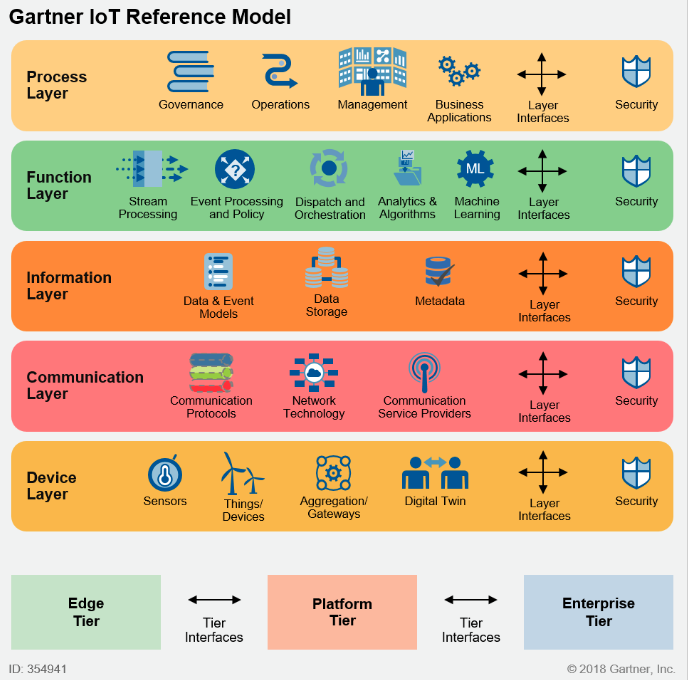
\includegraphics[width=75mm,scale=0.75]{Figures/gartnerIoT}
	\decoRule
	\caption[Gartner]{gartnerIoT1}
	\label{fig:gartnerIoT}
\end{figure}
\section{Prototyping (1-2p)}
//Proof of concept, MvP, Rapid Prototyping
\section{Front-End}
//Should I talk about other options too? (also in the following sections)
 Reactjs is an Open-Source Javascript-Libary.
After developing Reactjs in 2011, Facebook soon discovered that it's performance was faster than other implementations of its' kind and made it Open-Source in 2015. 
At present, React is used by major companies for their front-end like Airbnb, Netflix and Reddit \parencite{reactjsUsers}. 
In this years' Stackoverflow-Survey, React came third in "Most Popular Framework, libary or Tool" \parencite{stackOverflowSurvey}. 
This year, over 100,000 developers participated in the survey. 
React is designed for building User-Interfaces. Other libaries % \parencite{reactjsAngularVue} 
use the same concepts but Reactjs is currently the most popular one.
A lot of libaries are available for react. 
It's main concepts are:
\begin{description}
    \item[Components] \hfill \\
    React motivates its' users to write encapsulated components with single responsibilities. Components combine the HTMl-markup and Javscript-functionality of a responsibility. They are supposed to reusability. %erhöhen
    \item[Composition] \hfill \\
    The user can reuse and composite elements as he needs to. The isolated components makes code easier to maintain. 
    \item[Uni-Directional Dataflow] \hfill \\
            Properties should not be changed in other components, but passed down as read-only variables. 
            React doesn't want children to affect their parent components. That makes maintainability easier, as there's a clear downward structure in a well designed React project.
            If a user needs to pass changes to a parent component, it's executed with callbacks, or, for more complicated architecture with a Flux-supporting libary like Redux.
    \item[Virtual Dom]\hfill \\
    A DOM%Reference to Abkürzung 
    is a logical structure of documents in HTML, XHTML, or XML formats. 
    Web browsers are using layout engines to transform or parse the representation HTML-syntax into document object model that we can see in a web browser.
    Usually, when one of these elements changes, the whole structure has to be calculated again. 
    React uses a Virtual DOM as a negiator to enable calculating only the parts that need calculating. That's also possible because of Reacts' isolated component structure.
    \item[JSX]  JSX, short for Javascript XML, is an implementation of Javascript which is usually used to write in ReactJs. 
    It looks a lot like HTML but enables Javascript functionality. Javascript functionalities can be used by putting them in curly brackets ("{}").
\end{description}
\section{Communication}
%Socket.io
Socket.io is a Javascript-Libary designed for realtime communication. 
The server-side is developed for specifically for Node.js wheras for the client different implementations (e.g. .Net, Swift, C++)\parencite{socketioClients} are available.
It enables a bi-directional communication channel between a client and a server and offers a fallback mechanism to long polling when WebSockets are not available.
Once a connections is established it's maintained and uses a diminishing small amount resources to communicate. 
It uses an event-based system where one participant listens and another emits an event. 
Both Client and Server can emit and listen for events.
\section{Middleware}
%Talk about Node.js
Node.js is an open-source, cross-plattform, javascript-runtime-enviroment. 
With 49.6\% it is this years "Most Popular Framework, Libary or Tool" on this years Stackoverflow-survey \parencite{stackOverflowSurvey}.
According to Google Trends, interest is rising since 2012\parencite{gogleTrendNode}.
One explanation for that might be that it's written in Javascript. 
The transation for front-end Javascript developers to developing back-end is eased, which saves companies learning costs.
Node.js is estimated to have a high learning curve \parencite{nodeLearningcurve}.
It uses an event-driven architecture which operates on a single threaded event loop using non-blocking I/O calls.
Commands use callbacks to signal they are completed or failed. 
A downside is, that it doesn't allow vertical scaling by increasing the number of CPU cores of the machine it is running on. 
On CPU-intensive applications, that might become a problem - but modules like IPC or pm2 can add that functionality.
Node.Js commands are non-blocking and execute concurrently or in parallel. 
It's build on the Google V8 JavaScript engine which compiles Javascript to machine code instead of interpreting it in real time. 
That makes it faster than other engines.
There are thousands of open-source libaries and web frameworks. 
\section{Device}
%Talk about Arduino implementation
Arduino is a micro-controller-company from italy which was founded in 2005. It's is completely Open-Source and supplies everyone with it's own IDE \parencite{arduinoIDEDownload}.
The IDE works with nearly all micro-processors on the market, % gegeben the developer published a %entsprechende libary.
The Arduino (and comperable micro-processors) are programmed in C. 
\section{Back-End}
%Talk about postgres
We decided to use PostgreSQL for our database-back-end. Postgres is a light-weight open-source object-relational database system. 
Companies like Netflix, Spotify or Instagram \parencite{postgresUsers} rely on the flexible database system which allows SQl and noSQL design.
It's easy to set-up and maintain. 


%Even though, only 26\% of IoT-Projects in companies are judged to be a complete success 
%\parencite{ciscoresearch}. The reasons are as numerous as they are diverse. 
%Lack of knowledge, lack of planning, inconsistent standards and legacy architectures within the project are only some mentioned by the Cisco survey.
%A McKinsey report \parencite{mcKinsey} in 2015 stated that most IoT adopters fail to use their data or derive just a small part of its value.
